\subsection{Data View}
Som nævnt tidligere, så er meget af usermodellen givet på forhånd i Identity Framework. Derfor har projektgruppen altså ikke haft behov for at tilføje password, username, og email i usermodellen. Der er dog nogle attributer som skulle tilføjes, som kan ses på ER modellen på figur \ref{fig:ER_Model_User}:

\begin{figure}[H]
    \centering
    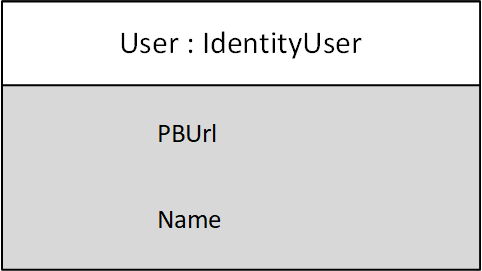
\includegraphics[width=0.45\linewidth]{09_Arkitektur/User/Images/User_DatabaseModel.png}
    \caption{User ER Model}
    \label{fig:ER_Model_User}
\end{figure}

Som der kan ses er der blevet tilføjet et Navn, som er en brugers nickname. Derudover er der sat en string ind til PBUrl. Ud over dette er der blevet lavet 4 relations til entiteterne Groups, WallPosts, GroupsAdministrators samt OwnerGroups.

\mini{Tjek om WallPosts skal fjernes}
